\documentclass[a4paper,11pt]{article}
\usepackage[a4paper,margin=1in]{geometry} % Adjust margins
\usepackage{tcolorbox}
\usepackage{listings}
\usepackage{xcolor}
\usepackage{amsmath}
\usepackage{graphicx}

\definecolor{codegray}{rgb}{0.9,0.9,0.9}
\definecolor{darkblue}{rgb}{0,0,0.5}

\lstdefinestyle{mystyle}{
    backgroundcolor=\color{codegray},   
    commentstyle=\color{darkblue},
    keywordstyle=\color{blue},
    numberstyle=\tiny\color{gray},
    stringstyle=\color{red},
    basicstyle=\ttfamily\footnotesize,
    breaklines=true,
    numbers=left,                    
    numbersep=5pt,                  
    showspaces=false,                
    showstringspaces=false,
    showtabs=false,                  
    tabsize=4
}
\lstset{style=mystyle}
\newtcolorbox{definitionbox}[1]{colback=blue!5!white,colframe=blue!75!black,title=#1}

\title{\Huge Turneu de E-Sports}
\author{Cocu Matei-Iulian}

\begin{document}

\maketitle

\section{Descrierea modelului și a regulilor de funcționare:}
\quad Modelul de date va gestiona informații legate de organizarea și desfășurarea unui \textbf{turneu de Counter Strike 2}, un joc First-Person-Shooter multiplayer competitiv în care două echipe a câte 5 jucători fiecare își demonstrează abilitățile strategice și practice.
Un asemenea \textbf{eveniment} este format din mai multe \textbf{stadii (etape)} eliminatorii,
la care participă multiple \textbf{echipe}, compuse la rândul lor din \textbf{membrii}. Echipele pierzătoare sunt progresiv eliminate, acest proces fiind repetat până când se ajunge în finala turneului, printr-un sistem de \textbf{meciuri} care pot conține mai multe \textbf{hărți} și sunt comentate și analizate de către \textbf{comentatori}. Evenimentul în sine, cât și echipele, pot fi sprijinite financiar de către \textbf{sponsori}. Bineînțeles, fiecare eveniment are o anumită sumă cumulată de \textbf{premii} de împărțit participanților, în funcție de locul obținut pe parcursul turneului.

\quad Într-un context mai detaliat, fiecărei hărți îi este asociată un \textbf{jurnal}; cât despre participanții la acest eveniment, fiecare membru are un anumit \textbf{rol} în echipă, având, de asemenea, și un \textbf{istoric} personal al echipelor anterioare din care a făcut parte. Bineînțeles, sponsorii evenimentului, cât și ai echipelor participante au întocmite \textbf{contracte} cu organizațiile responsabile de acestea.

\section{Restricții (constrângeri de funcționare) - se implementează la nivel de cardinalitate:}
\begin{itemize}
    \item Un eveniment are cel puțin un stadiu de desfășurare.
    \item Un eveniment are cel puțin un sponsor, dar un sponsor nu trebuie neapărat să suporte financiar un anumit eveniment.
    \item Un eveniment are valabile mai multe premii de acordat echipelor participante, în funcție de stadiul în care acestea au ajuns.
    \item În cadrul unui stadiu trebuie să participe cel puțin două echipe, iar o echipă trebuie să participe la cel puțin un stadiu.
    \item O echipă poate să aibă zero sau mai mulți sponsori, iar un sponsor poate suporta financiar zero sau mai multe echipe participante.
    \item Un stadiu trebuie să aibă în componența acestuia cel puțin un meci de jucat.
    \item Un meci poate fi jucat doar între două echipe.
    \item Un meci poate fi comentat de către mai mulți comentatori, iar un comentator poate comenta mai multe meciuri din cadrul unui eveniment.
    \item Un meci trebuie să conțină cel puțin o hartă jucată, ajungând până la un număr maxim de 5 hărți jucate într-un singur meci (acest număr maxim depinde, bineînțeles, de tipul stagiului curent).
    \item O echipă este eligibilă dacă are minim 5 membrii valabili pentru a participa la turneu (este permisă o singură rezervă per echipă). De asemenea, o echipă poate avea, opțional, și un membru special, un antrenor, care nu participă în mod direct în meciurile jucate (în cazuri extreme, antrenorul poate, totuși să fie considerat și jucător în sine, participând în mod direct în cadrul unui meci).
    \item Un membru poate activa, bineînțeles, la o singură echipă. De asemenea, un membru poate avea în echipa curentă un singur rol asignat acestuia (în ideea în care un membru nu poate avea mai multe roluri simultan).
    \item Cu toate acestea, jucătorii pot avea mai multe echipe din care să facă parte, schimbându-și organizația la care joacă, participând la alte evenimente sub numele acesteia; vice-versa, o echipă (organizație) poate avea mai mulți diferiți jucători, totul fiind bazat pe o relație contractuală ce ține cont de anumitele posibile evenimente la care echipa poate participa.
\end{itemize}

\section{Proiectarea diagramei Entitate-Relație}
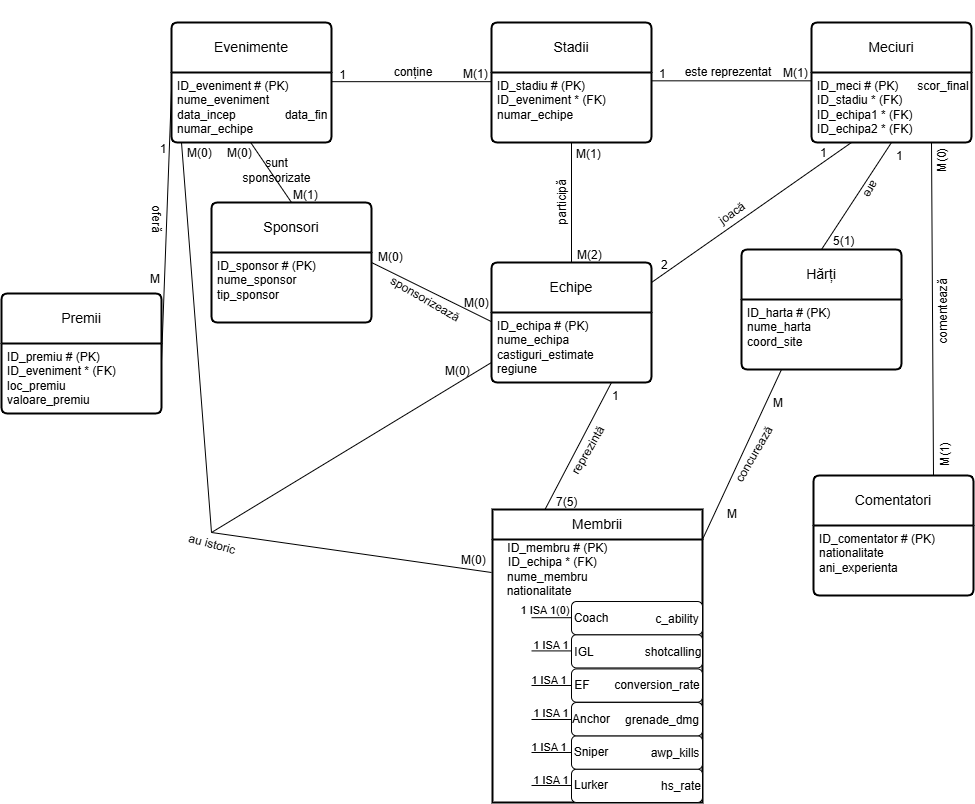
\includegraphics[scale=0.515]{diagramaER.drawio.png}

\subsection{Descrierea entităților}

Pentru modelul de date referitor la \textbf{turneul de CS2}, structurile EVENIMENTE, PREMII, SPONSORI, STADII, ECHIPE, MEMBRII, MECIURI, HĂRȚI, COMENTATORI reprezintă entități.

\subsubsection{Entitate independentă}
\quad \textbf{EVENIMENTE} \texttt{$=$} turneele de Counter Strike 2 organizate și distribuite public. Cheia primară a acestei entități este \textbf{ID\_eveniment}.

\subsubsection{Entitate dependentă}
\quad \textbf{PREMII} \texttt{$=$} recompensele monetare acordate de către organizatorii evenimentului echipelor participante, în funcție de poziția acestora în ierarhie la finalul turneului (stadiul în care a ajuns echipa). Cheia primară a acestei entități este \textbf{ID\_premiu}. Această entitate depinde de entitatea principală, \textbf{EVENIMENTE}, deoarece fără un eveniment valid, nu pot exista premii acordate.

\subsubsection{Subentitate}
\quad În diagrama expusă anterior, singura entitate ce conține subentități este \textbf{MEMBRII}, acestea reprezentând, bineînțeles, rolurile (specializările) acestora în cadrul echipei.

\textbf{EF} \texttt{$=$} descrie rolul de \emph{Entry Fragger} într-o echipă. Jucătorul cu acest rol este, de obicei, cel care preia inițiativa pe tabela de joc, fiind cel care caută o victimă cât de repede posibil în fiecare rundă a meciului. 
Cheia primară a acestei entități este preluată de la entitatea principală \textbf{MEMBRII}: \textbf{ID\_membru}. 

\subsection{Descrierea relațiilor}
\subsubsection{Relație many-to-many}
\textbf{SPONSORI\_ECHIPE} \texttt{$=$} relație dintre entitățile SPONSORI și ECHIPE, reprezentând echipele suportate financiar de anumiți sponsori. Relația are cardinalitate minimă 0:0 (o echipă nu trebuie să aibă nici un sponsor, iar un sponsor nu trebuie să fie asociat cu nici o organizație de Counter Strike) și cardinalitatea maximă M:M (o echipă poate avea mai mulți sponsori în același timp, iar un sponsor poate avea contracte cu mai multe echipe în același timp).

\subsubsection{Relație de tip 3}
\textbf{JUCATORI\_reprezintă\_ECHIPE\_la\_EVENIMENTE} \texttt{$=$} relația ternară dintre entitățile MEMBRII, ECHIPE și EVENIMENTE, ce reprezintă istoricul unui jucător la o echipă în relație cu posibile multiple evenimente. Un jucător poate reprezenta multiple echipe pe parcursul unei anumite perioade de timp, la multiple evenimente, o echipă poate fi compusă din diferiți membri pentru orice eveniment la care participă (relație cu cardinalitatea maximă \textbf{M} și cea minimă \textbf{0} (un jucător nu trebuie să facă parte dintr-o echipă, poate fi retras, sau doar inactiv, și nu este obligat să-și reprezinte echipa din care face parte la nici un eveniment, în timp ce o echipă nu trebuie să participe la un anumit eveniment neapărat) pentru toate cele 3 entități).

\subsubsection{Relație one-to-one}
\textbf{ECHIPE\_joaca\_MECI} \texttt{$=$} relație de cardinalitate fixă 2:1 între entitățile ECHIPE și MECIURI, fiind necesare fix două echipe pentru desfășurarea unui meci din cadrul unui stadiu.

\subsubsection{Relație one-to-many}
\textbf{EVENIMENT\_are\_STADII} \texttt{$=$} relația dintre entitățile EVENIMENTE și STADII, reprezentând dependența unui stadiu de un eveniment (ideea că un eveniment se împarte în mai multe stadii: faze eliminatorii, sferturi de finală, semifinale, și, în sfârșit, finală). Cardinalitatea maximă este 1:M, având în vedere că un singur eveniment poate avea cât de multe stadii sunt necesare (și, bineînțeles, un stadiu nu poate aparține mai multor evenimente), iar cardinalitatea minimă este 1:1, având în vedere faptul că un stadiu trebuie obligatoriu să aparțină unui eveniment, iar un eveniment valid trebuie să conțină cel puțin un stadiu (un singur meci, o finală disputată între două echipe, în cel mai restrâns caz). 

\subsection{Descrierea atributelor}
\subsubsection{Atributele unei entități independente}
Entitatea independentă \textbf{EVENIMENTE} are ca atribute:
\begin{itemize}
    \item nume\_eveniment \texttt{$=$} variabilă de tip șir de caractere, de lungime maximă 50, care reprezintă numele evenimentului (\textbf{VARCHAR2(50)})
    \item data\_incep \texttt{$=$} variabilă de tip dată calendaristică, care reprezintă data începerii turneului (ziua începerii primului stadiu) (\textbf{DATE})
    \item data\_fin \texttt{$=$} variabilă de tip dată calendaristică, care reprezintă data terminării turneului (ziua finalei) (\textbf{DATE})
    \item numar\_echipe \texttt{$=$} variabilă de tip întreg, de lungime 3, care reprezintă numărul de echipe participante la eveniment (\textbf{NUMBER(3)})
\end{itemize}

\subsubsection{Atributele unei subentități} 
Subentitatea \textbf{ANCHOR} a entității \textbf{MEMBRII} are un singur atribut adițional, moștenind restul atributelor (și bineînțeles, cheia primară și cheile externe) de la aceasta.
\begin{itemize}
    \item nume\_membru \texttt{$=$} variabilă de tip șir de caractere, de lungime maximă 30, ce reprezintă porecla jucătorului (\textbf{VARCHAR(30)})
    \item nationalitate \texttt{$=$} variabilă de tip șir de caractere, de lungime maximă 25, ce reprezintă țara din care provine jucătorul (\textbf{VARCHAR(25)})
    \item ID\_echipă (FK) \texttt{$=$} variabilă de tip întreg, de lungime 6, reprezintă cheia externă ce face referire la cheia primară \textbf{ID\_echipă} din entitatea \textbf{ECHIPE} (\textbf{NUMBER(6)})
    \item grenade\_dmg (atribut specific subentității) \texttt{$=$} variabilă de tip întreg, de lungime 6, reprezintă daunele provocate de jucător în materie de grenade aruncate (\textbf{NUMBER(6)})
\end{itemize}

\subsubsection{Atributele unei relații}
Relația ternară (de tip 3) dintre entitățile EVENIMENTE, ECHIPE și MEMBRII, \textbf{JUCATORI\_reprezintă\_ECHIPE\_la\_EVENIMENTE}, ce reprezintă istoricul unui jucător la o echipă în relație cu posibile multiple evenimente (mai simplist, statisticile unui jucător, reprezentant al unei echipe, în cadrul unui eveniment), are ca atribute:
\begin{itemize}
    \item kill\_count \texttt{$=$} variabilă de tip întreg, de lungime 3, reprezintă câte entități de jucător a omorât membrul, cumulat, pe tot parcursul evenimentului
    \item assist\_count \texttt{$=$} variabilă de tip întreg, de lungime 3,reprezintă de câte ori a asistat membrul, cumulat, pe tot parcursul evenimentului
    \item death\_count \texttt{$=$} variabilă de tip întreg, de lungime 3, reprezintă de câte ori a murit membrul echipei în joc, cumulat, pe tot parcursul evenimentului
\end{itemize}

De asemenea, conține și cheile externe:
\begin{itemize}
    \item ID\_eveniment  (FK) = variabilă de tip întreg, referință către cheia primară \textbf{ID\_eveniment} din entitatea \textbf{EVENIMENTE} (\textbf{NUMBER(5)})
    \item ID\_echipa (FK) = variabilă de tip întreg, referință către cheia primară \textbf{ID\_echipa} din entitatea \textbf{ECHIPE} (\textbf{NUMBER(6)})
    \item ID\_membru (FK) = variabilă de tip întreg, referință către cheia primară \textbf{ID\_membru} din entitatea \textbf{MEMBRII} (\textbf{NUMBER(7)})
\end{itemize}

\section{Diagrama Conceptuală}
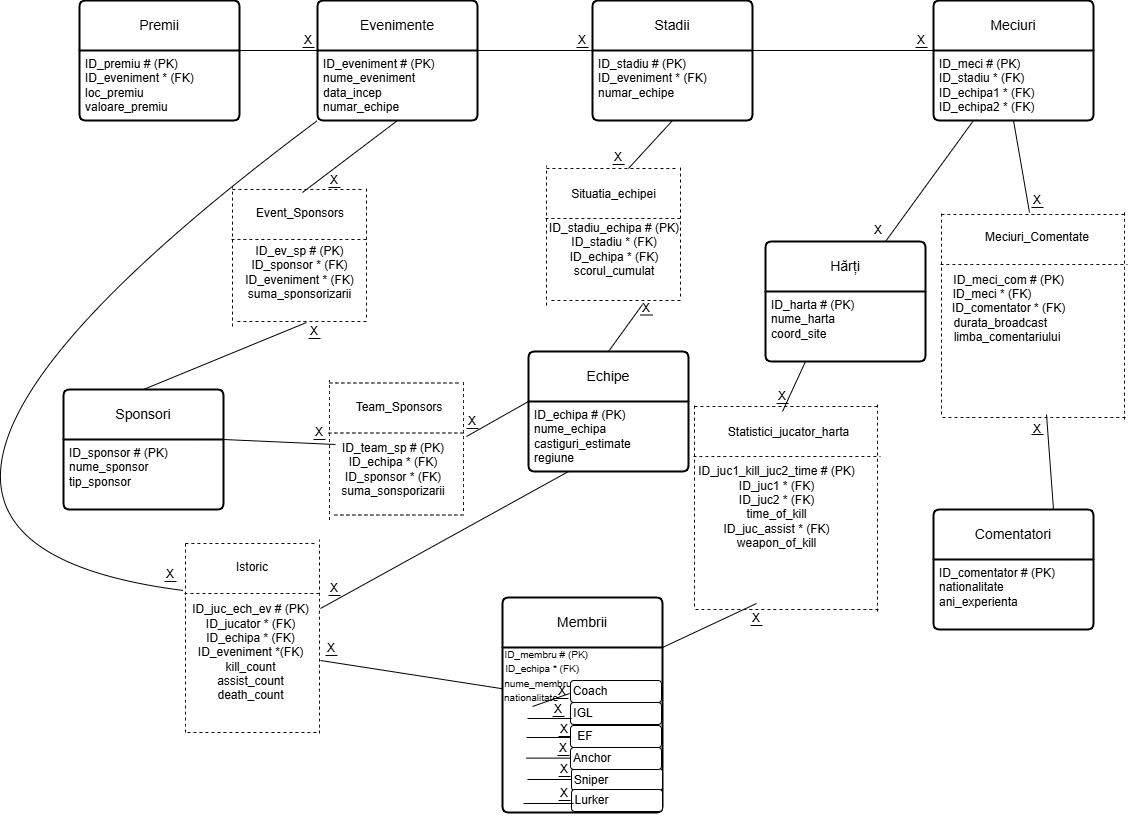
\includegraphics[scale=0.46]{diagramaConcept.drawio.png}

\section{Schemele relaționale ale Diagramei Conceptuale}
\subsection{Tabel independent}
\textbf{EVENIMENTE}(ID\_eveniment\#, nume\_eveniment, data\_incep, data\_fin, numar\_echipe)

\subsection{Subtabel}
\textbf{SNIPER}(ID\_membru\#, ID\_echipa*, nume\_membru, nationalitate, awp\_kills)

\subsection{Tabel asociativ}
\textbf{ISTORIC}(ID\_juc\_ech\_ev\#, ID\_jucator*, ID\_echipa*, ID\_eveniment*, kill\_count, assist\_count, death\_count)

\end{document}